%\underline quotation vokabulary page 39-40
%\Large They say/I Say
%\textbf Vokab list
\section{Oil Consumption}
To the energy market there are participating suppliers, concurring against each other, 
making use of various natural sources and technical methods, as well as consumers, and users on the other
side, using the energy to run their own business and gaining prosperity obeying the rules of capitalism \cite{capitalism}.
\par
Before I present some specific data I do want to mention that, because the worldwide pandemic has "dramatical" \cite[3]{IEAApril} effects on the energy market, 
this currently degraded demand, which is "erasing almost a decade of growth," how the International Energy Agency describes it in the newest oil market report \cite{IEAApril},
will probably not represent the future trend I decided to use data from the last few years, therefore.
According to the International Energy Agency, in the year 2017, 41\% of the total energy demand was performed by oil combustion.
The other fossil energy sources contributed with 36\% for coal and 31\% for natural gas. 
Biowaste is providing almost 11\%, nuclear power 6\% and all others together 6.2\% of the contributions \cite{WEO_P_C}.
\par
The consumers are dividing in industry, transportation, housing, and others (\figref{fig:IEA_consumption}), which might be important to keep in mind
when we are talking about potential technical solutions for saving fossil resources in the following chapters.
For instance, the International Energy Agency is aware of the problem
that the major used renewable power supplies are producing electric power,
which poses difficulties for implementation in industries or transportation, 
where high energy volume or energy density is especially important \cite{IEA_Industries}.

\begin{figure}
  \centering
  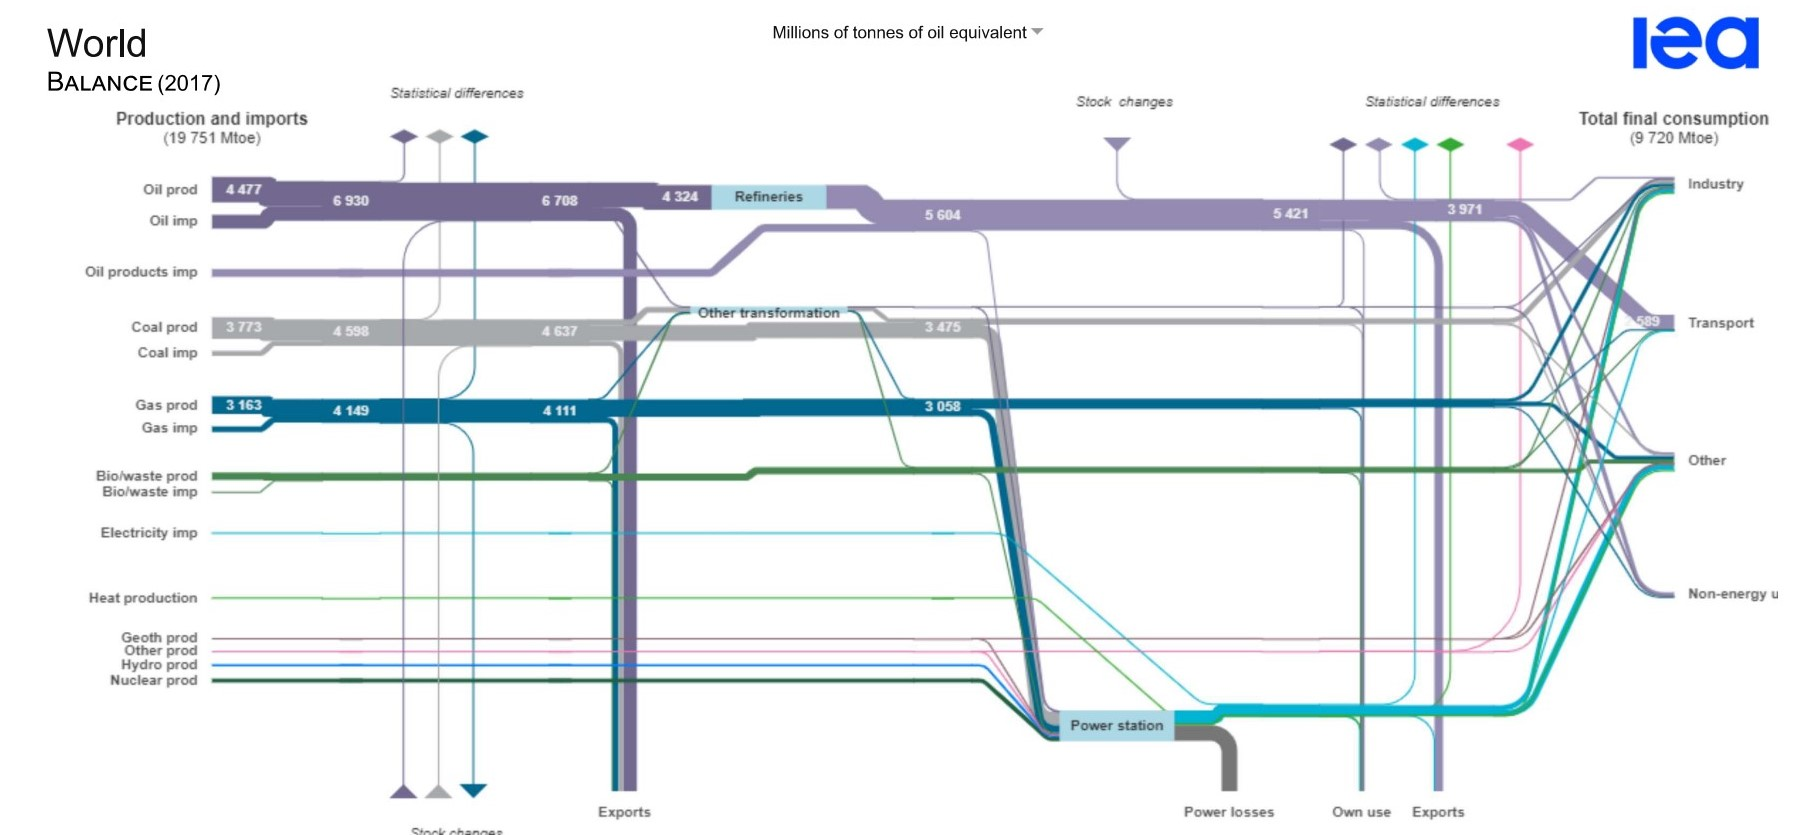
\includegraphics[width=0.85\textwidth]{graphics/IEA_Prod_and_Cons_2017.jpg}
  \caption{Breakdown of worldwide oil prdoduction in units of million tonns of oil equivalent. The data apply to 2017\cite{WEO_P_C}.}
  \label{fig:IEA_production}
\end{figure}

\begin{figure}
  \centering
  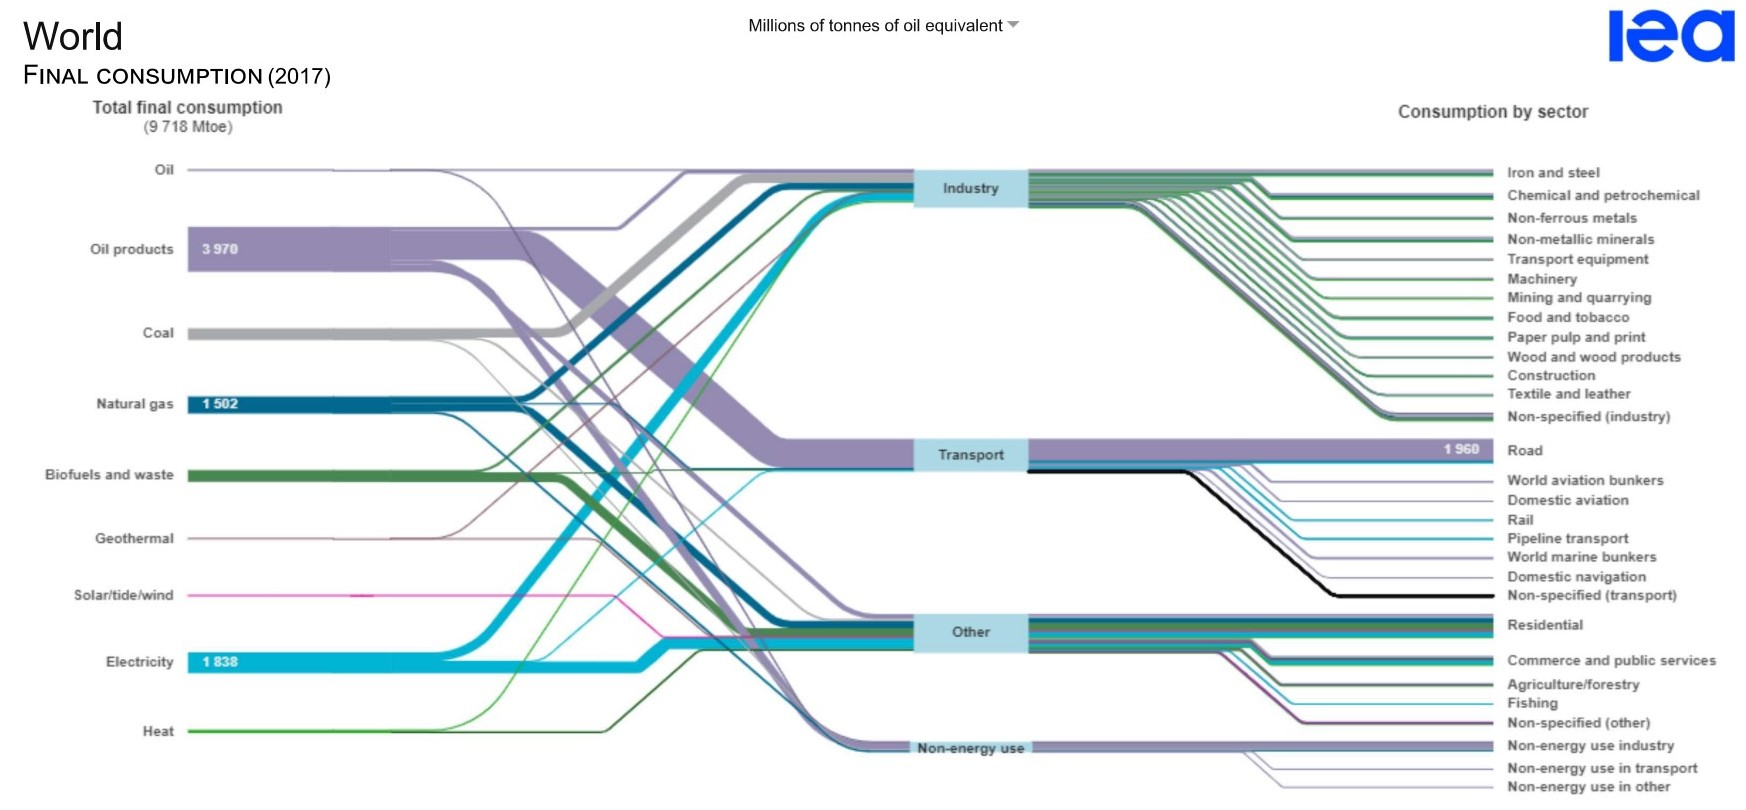
\includegraphics[width=0.85\textwidth]{graphics/IEA_Cons_2017.jpg}
  \caption{Breakdown of worldwide oil consumption in units of million tonns of oil equivalent. The data apply to 2017 \cite{WEO_P_C}.}
  \label{fig:IEA_consumption}
\end{figure}


\section{UN Climate and Energy Goals}
\label{sec:UN}
The United Nations are \textbf{aware} of the danger of human-made climate change, so they decided to not exceed global 
average heating of 2.0\degree C compared to preindustrial eras \cite{UN_Plan}. 
This upper limit, called out by the UN, is \underline{asserted} as the biggest possible change, "without the risk of causing worldwide irreparable damage, endangering human civilization" \cite{UN_Climate_Goals}.
However, to reach this goal requires reductions of carbon emissions, and later steming them for all time, using a net invoice.
According to Baake, at least half of the known fossil oil reserves have to be held untouched, to not
pass the CO2 limit correlated with the 2\degree C goal \cite{Industries}. 
This, in the end, grounds my scenario background in which I am questioning what will happen, 
where 25 years of fossil-based economic growth are left \cite{Bible}.
The UN, and even German ministers see decreasing expenses of renewable energies as the most natural and
the easiest way to implement these \cite{UN_Plan}; \cite{Industries}. 
Renewable energy sources would become the new standard, 
while fossil fuels would cover only cases in which the technology is not providing any alternative,
or the use of renewable power is expensive disproportionately \cite{Industries}.
{\Large Furthermore, the UN is pointing out especially, that} fossil resources, if they are used, 
should be used most efficiently \cite{UN_Plan}. 
To reach this \textbf{goal}, huge changes like centralization of energy supplies in developing countries are needed \cite{UN_Plan}.
{\Large Although the UN determines} following the actual trend of energy production and consumption would lead in surpassing the 2\degree C limit greatly,
especially when we are aware that growing prosperity comes along with more energy demand \cite{prosperity}, the authors of the UN Climate Plan see hope in so-called
"carbon caption systems" \cite{UN_Plan}. 
In fact, this strategy could prevent the global civilization from natural disasters caused by climate change \cite{UN_Climate_Goals}, 
but the UN gives no specific answer for the scenario I am questioning, not double-checking, that it is not preventing the world economy from running out of fossil 
energy sources, which would come with an economic and geopolitical blackout \cite{Bible}.
\par
Another hurdle the International Energy Agency is \underline{suggesting} is that available sustainable technologies are
most notably implemented in less energy-consuming sectors such as private housing and mobility (\figref{fig:IEA_consumption}), 
rather than in heavy industry or transportation \cite{WEO_P_C}.


% \cite{WEO}
% \cite{Algae}
\section{Example of Sweden}
\label{sec:Sweden}
The UN is providing an approximate direction, but, as the UN declares, the real implementation has to be adapt filigree in a countries 
geography, energy grid, and economic system. 
To find out what is possible by now, I pick out the example of Sweden, {\Large which is, as some people might say}, 
one of the best-developed countries on earth, not only in social but also in sustainable standards \cite{Sweden_happy}.
And indeed, we can find a governmental paper elaborating detailed plans about how Sweden could become an oil-free society \cite{Sweden}.
This \underline{call} for action is, by the way, less \underline{pleaded} by the climate \textbf{debate}, 
but more by the need to be independent and peaceful with other countries \cite[2]{Sweden}.
Very interesting is that the government plan has been set up already in 2006 with the deadline of 2020, so we can \textbf{evaluate} the success.
\par
However, the set strategies, set out in the Committee's paper, have been reducing energy consumption in industry and private mobility by expanding the IT-infrastructure and making public transportation more convenient.
Also, {\Large according to} the Committee, fossil energy sources should not be used for residential heating.
The Agency \underline{consedes} that several industry branches are not suitable to run on electricity, so it \underline{suggests} that fossil oil would be replaced by biofuels.
They also {\Large claim that} electricity-driven heaters could replace the gas-driven ones \cite[4]{Sweden}.
\par
Until the efficiency could be improved by implementing new technologies, the Committee also \underline{acknowledges} the rebound effect.
This effect describes the growing net consumption of energy because of the growing demand for higher living standards, although there are improvements in efficiency \cite[5]{Sweden}.
To counteract a growing net consumption of fossil resources as a result of this effect, adjusted tax laws, education, and nationwide "save energy" campaigns are \underline{proposed} as a strategy \cite[5]{Sweden}.
\par
"On the other hand side, the methods of energy production have to change." thus the Committee \cite[14]{Sweden}. 
Sweden has a lot of forests, so the committee is suggesting to use this biomass for heating \cite[14]{Sweden}.
Further, electricity should be produced by offshore wind-parks and nuclear energy instead of coal combustion \cite[14-15]{Sweden}.
\par
The data from 2020 are not available by now, but these from 2018 are. 
\figref{fig:sweden_2018} shows, that Sweden needs only 10 percent of fossil resources too supply their energy demands.
At least 38 percent of the energy is produced by hydro-generators and 20 percent by nuclear reactors. 
\begin{figure}
  \centering
  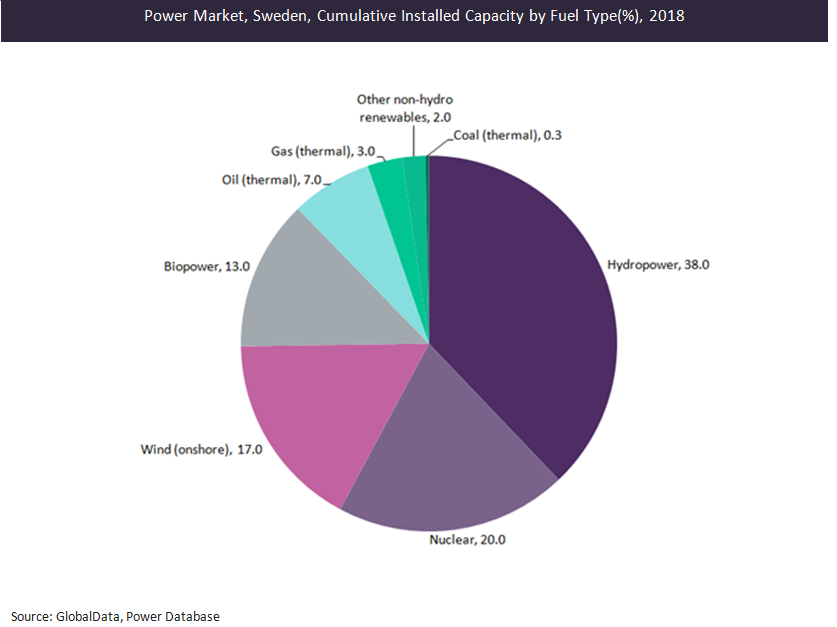
\includegraphics[width=0.85\textwidth]{graphics/sweden_2018.png}
  \caption{Breakdown of Swedish energy consumption in percent. The data apply to 2018. \cite{sweden_2018}}
  \label{fig:sweden_2018}
\end{figure}
\par
If all counties would economize as Sweden, there might be no big problem in twenty-five years and there would be no oil anymore because the dependency is so small.
We have to admit, that these strategies are very specific for a country like Sweden, where there are a lot of forests and coasts \cite{Sweden}.
Hence, we will spotlight strategies made for other regions too.
\par
At the and I would like to mention a very specific answer witch the committee has given in their declaration:
Although Sweden is facing the goal to reduce the oil consumption to a minimum, the committee objects the end of fossil resources, interestingly.
The sources might be harder to tap, and more expensive to run then they are now, but there is no expectation of an ever happening blackout \cite[7]{Sweden}.
At once, the committee does not object, that the negative impact of using these resources could gravely destabilize the worldwide economy.
This statement sheds a different light on the research question, where the statement of ending oil sources vanishes. 
Following this argumentation, counties would not prepare for an absence of oil, allowing to answer my main research question on the one hand side with: 
No, the countries are not preparing; but on the other hand side, with: 
But they don't have to, in order to prevent negative economic consequences.  
\par

\section{Example of New York}
\label{sec:NY}
As the UN (Section \ref{sec:UN}) proposes, solutions for worldwide independence of fossil fuels have to be found in small, individual scales.
And indeed cities like New York, built close by the water, might be especially interested in fasten the sustainability transformation of power supplies, 
in order to prevent damage caused by rising sea levels \cite{NY_Sea}. 
Especially New York is an interesting example because it is more representative relative to
weather conditions, more limited natural resources, and less free space, compared to the rather \textbf{unique} Sweden \cite{NY_average}.
\par
However that be, Standford researchers developed a plan of how New York could provide all their demand by their own, without using fossil sources until 2030.
More interestingly, they spare nuclear power, and also biomass in their version \cite[585]{NY_Jacobson}.
By using rooftops for installing photovoltaic, the required area for new installations can be reduced under 2 percent of the total state area \cite[590]{NY_Jacobson}.
The plan shows off that installing renewable energy sources, especially wind turbines, is even cheaper than to back on conventional power supplies \cite[592]{NY_Jacobson}.
\par
Hence, I would \textbf{assume}, that in a competitive market, the chances are good for implementing these techniques soon \cite{capitalism}. 
The final date of an oil-free New York could be surely deferred
because of still running coal- and oil-generators which did not reach their return of investment.
\par
Although these plans exit, showing up a less oil-dependent future, actual analysis from the year 2017 state that New Yorks energy is still produced
by gas and fossil oil products, by very major parts \cite{NY_2017}.
\par
The actual progress in New York reflects the UN statement, in which the future will not be oil-free, but rather will have implemented carbon capture systems, to reach the self-defined climate goals (Section \ref{sec:UN}).
\par
Nevertheless, {\Large Rosendahl argues, that} the papers of Jacobsen and others are clearly showing off a soon oil-free economy, with which she disagrees the UN made statement (Section \ref{sec:UN}).
She contradicts, fossil fuels would be needed for a stable energy market \cite[1]{NYT1}, pointing out the vast technical options 
given for countries and cities all around the world, implementing a cheap and efficient, sustainable power grid \cite[2]{NYT1}.

\section{Example of China}
\label{sec:China}
China is the biggest energy consumer in the world, using 30 billion oil equivalents of energy every year\cite{IEA_China_demand}.
The International Energy Agency reveals, that China will be the leader in implementing renewable energies, 
whereas most of the ever-growing demand will be covered by renewable energy systems \cite{IEA_China_overview}.
\par
But here, the rebound effect (Section \ref{sec:Sweden}) eventuates, which means that although the percentage for renewables in the total energy mix increases,
the absolute consumption of fossil resources, in China's case, especially coal and gas, will grow continually \cite[1480]{China_economy} \cite[1482]{China_economy} \cite{Sweden}.
The data are displayed in \figref{fig:china_mix}, whereby potential lower costs for more developed and efficient renewable energy sources, and the meanwhile increasing oil price is included in the scenario-calculation already \cite[1482]{China_economy}.

\begin{figure}
  \centering
  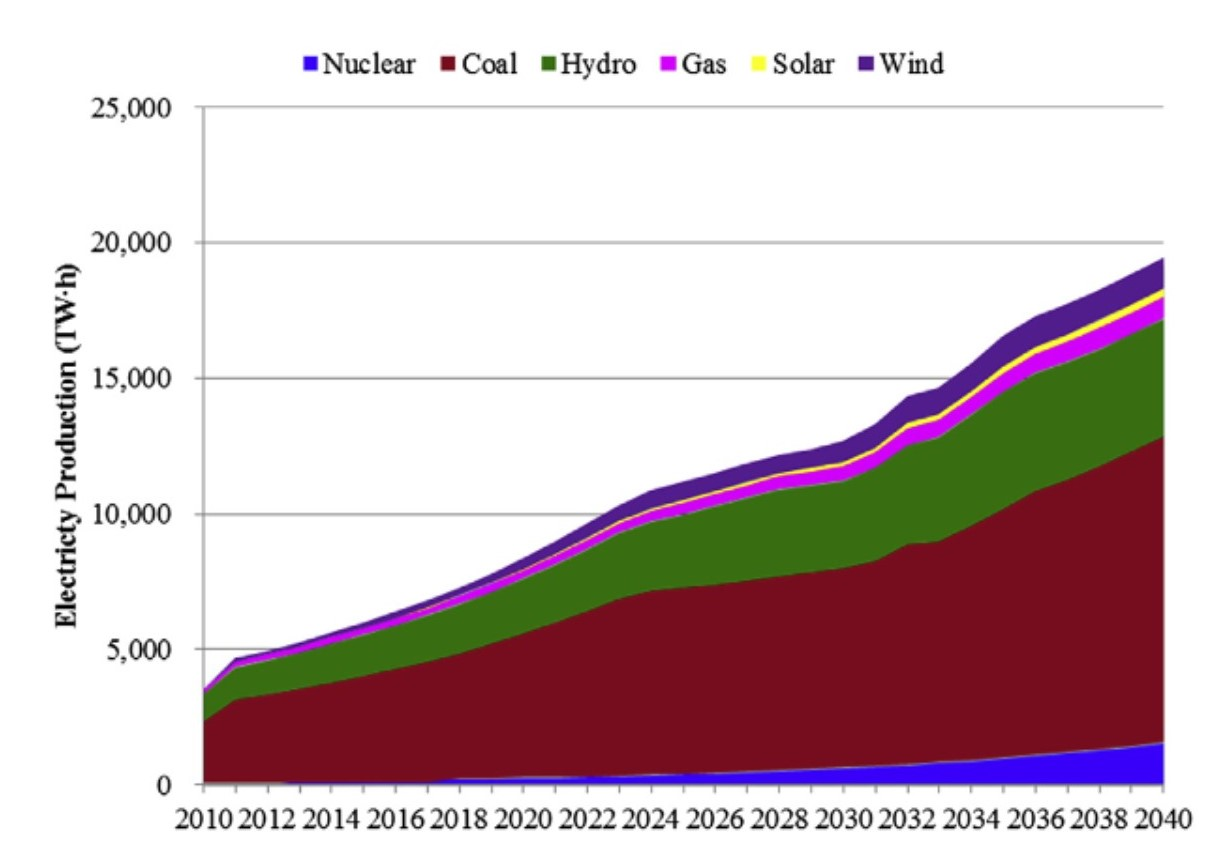
\includegraphics[width=0.85\textwidth]{graphics/China_mix.jpg}
  \caption{Chinas electricity production by type of fuel under the base case scenario for the period 2010 until 2040 \cite{UN_Climate_Goals}.}
  \label{fig:china_mix}
\end{figure}

\par
This development makes clear that sustainable energy politics are only possible with full consideration for ongoing economic growth and resilience.
Investments belonging to the past, like newly built coal-based power generators in China, will not be shut down before their return of investment is reached \cite[1577]{ChinaEvol}.
Generally, the "role of scientists has been reduced in the decision making process," according to Zhi \cite[1]{ChinaEvol}.
Sooner, innovation is seen as the best way for uncomplicated problem solving, 
wherefore China becomes a co-founder of the Clean Energy Ministerial founded in 2010 \cite{IEA_China_comment}. 

\section{Oil Companies}
\label{sec:BP}
BP, an oil and gas company, is publishing a detailed statistical review of worldwide energy supply every year \cite{BP}.
According to this report, as already mentioned in section (Section \ref{sec:introduction}), BP awaits the end of today's oil sources in 50 years.
Moreover, the company shares the idea, renewable energies are needed to make the energy market emission-free.
But they would not be able to provide the whole energy demand worldwide \cite[1]{BP}.
\par
The company is trying to decarbonize their production and products instead, to not pass the climate goals \cite{BP_renew}.
BP also invests in renewable energies, renaming themselves to "Beyond Petroleum" in 2001, looking towards sustainable energy sources \cite{BP_renew}.
%\cite{NYT1} Counterview Oil

\section{Prognosis}
\label{sec:prognosis}
Declining, as we see in \figref{fig:prognosis}, which is obtained from the paper \cite[633]{UN_Climate_Goals} there is no big agency, expecting a decreasing CO2 emission until 2040.
We also see, that the UN climate goals are expected to not be reached. 
This statement provides one of the main answers to the very first question about oil independence since we can assume that CO2 production correlates with fossil fuel consumption \cite{oil_comb} \cite{OILCombustion}.
It straightens out, that although there is an international agreement, nations are acting intending to improve their prosperity, nowadays based on consumption \cite{Sweden} \cite{capitalism} \cite[1577]{ChinaEvol}. 
Still, there are improvements in efficiency and integrations of sustainable energy sources detectable (\figref{fig:prognosis}), 
but vast not enough to avoid a pat situation where either the climate change is concussing 
worldwide infrastructure and economy \cite[3]{Sweden}, or the lack of fossil resources itself restrict the world's commerce seriously \cite{Bible}.
\par
{\Large However, some scientists object, that} since the effects of climate change will be aggravating enough, there will be a fast change in the worldwide energy 
supply. \cite{nuclear}
Because it will be too late for implementing sustainable systems like solar and wind using generators \cite{WEO}, the oil dependency, and the climate impact will be eluded with nuclear reactors,\underline{corroborates} Corner \cite[4828]{nuclear}.
Not electrified industry branches, such as long-distance transportation and aviation will be without any alternative \cite{WEO}.
Instead, the already mentioned carbon capture systems would become implemented \cite{UN_Plan}, decelerating the confrontation with a final oil lack \cite{nuclear}.

\begin{figure}
  \centering
  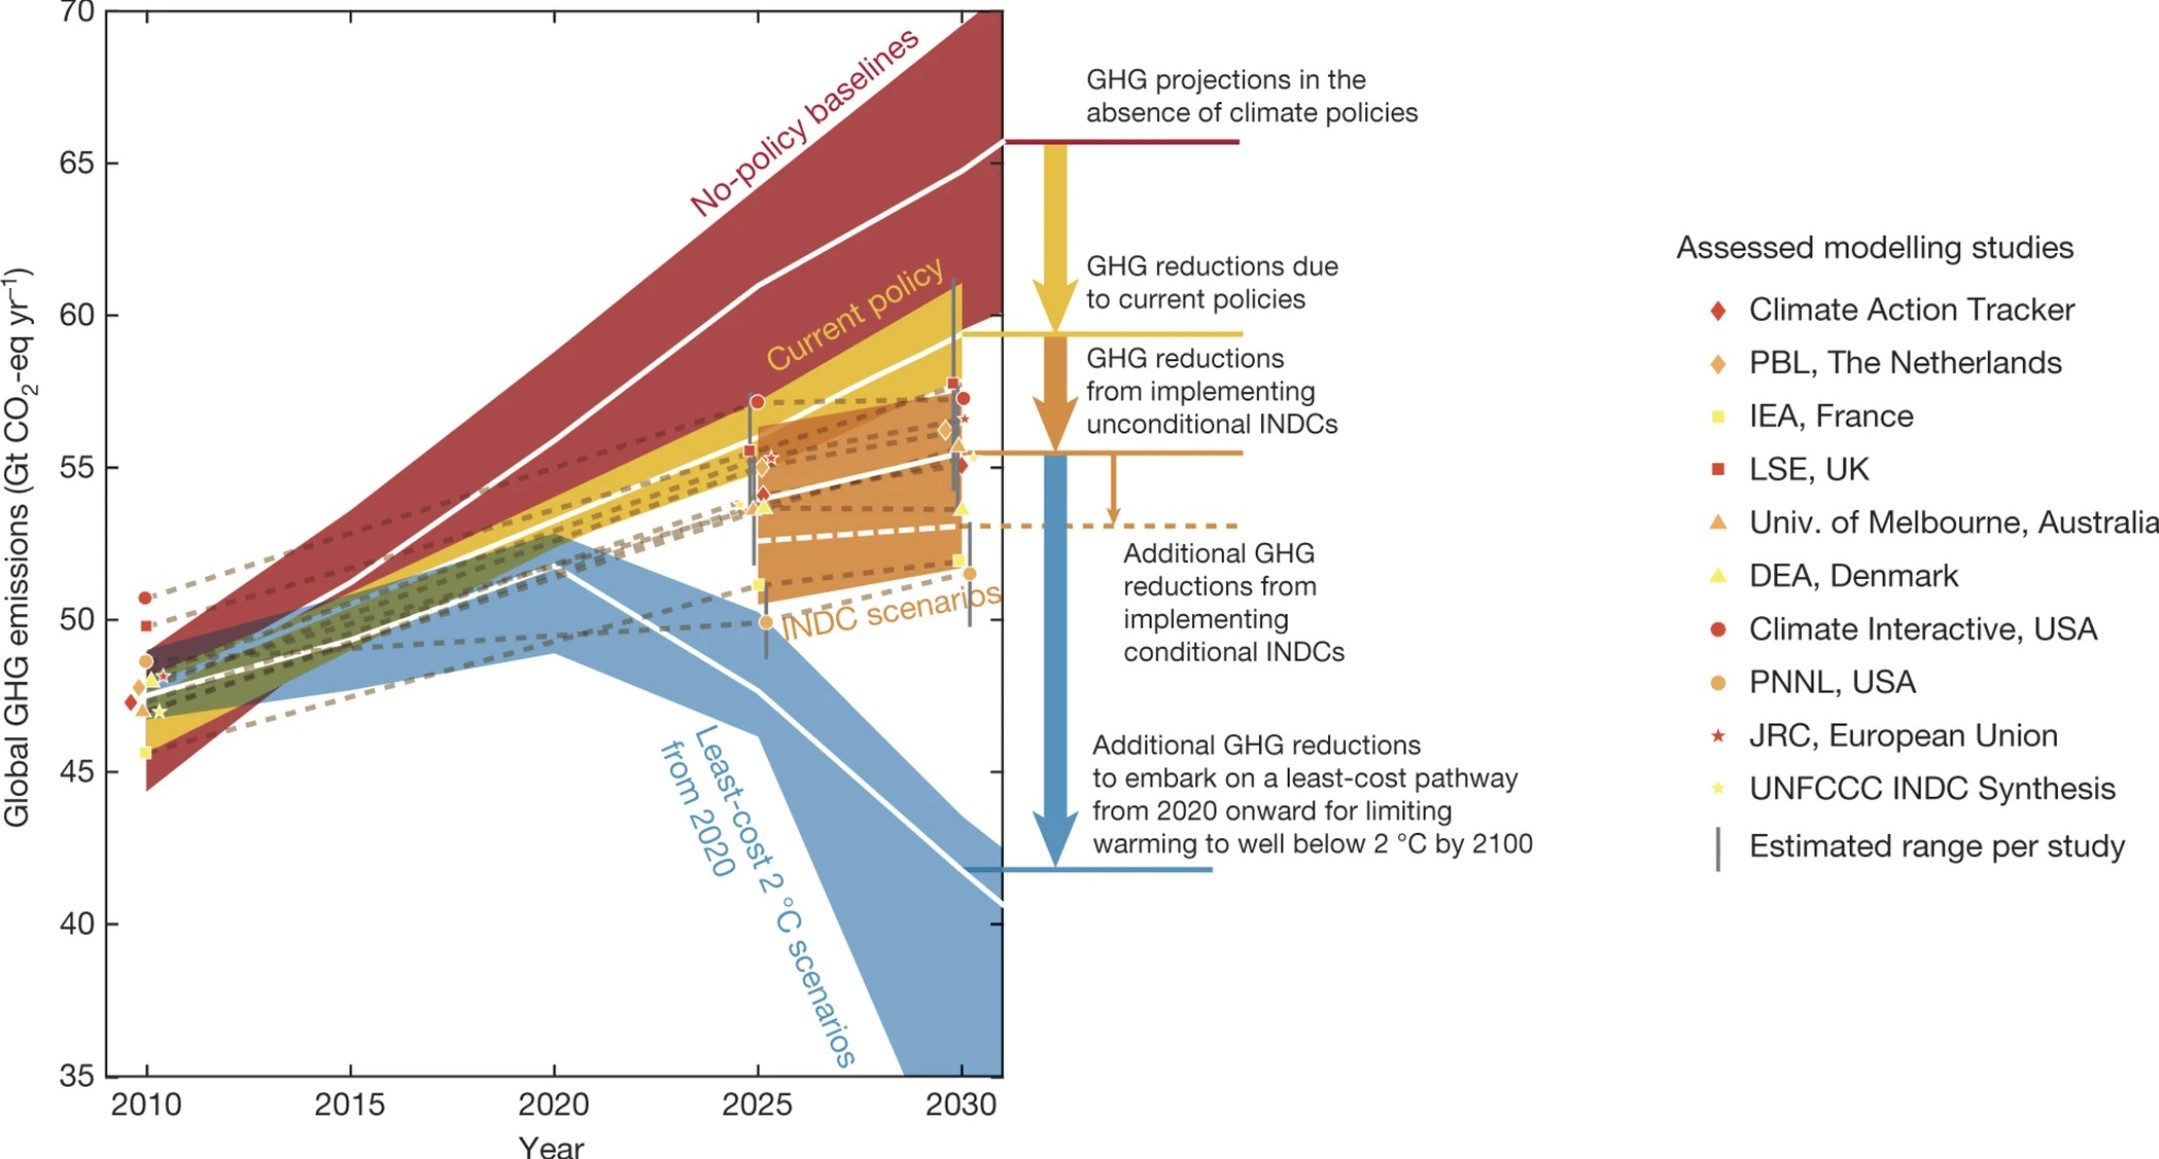
\includegraphics[width=0.85\textwidth]{graphics/politics_trend.jpg}
  \caption{2016 based data have been used to predict future CO2 emissions worldwide by different agencies and organizations. In addition, the graph, expected to reach the UN climate goals is listed. We can assume a correlation between CO2 emissions and use of fossil fuels \cite{UN_Climate_Goals}.}
  \label{fig:prognosis}
\end{figure}


